\PassOptionsToPackage{unicode=true}{hyperref} % options for packages loaded elsewhere
\PassOptionsToPackage{hyphens}{url}
%
\documentclass[ignorenonframetext,aspectratio=169,12pt]{beamer}
\usepackage{pgfpages}
\setbeamertemplate{caption}[numbered]
\setbeamertemplate{caption label separator}{: }
\setbeamercolor{caption name}{fg=normal text.fg}
\beamertemplatenavigationsymbolsempty
\usepackage{lmodern}
\usepackage{amssymb,amsmath}
\usepackage{ifxetex,ifluatex}
\usepackage{fixltx2e} % provides \textsubscript
\ifnum 0\ifxetex 1\fi\ifluatex 1\fi=0 % if pdftex
  \usepackage[T1]{fontenc}
  \usepackage[utf8]{inputenc}
  \usepackage{textcomp} % provides euro and other symbols
\else % if luatex or xelatex
  \usepackage{unicode-math}
  \defaultfontfeatures{Ligatures=TeX,Scale=MatchLowercase}
\fi
% use upquote if available, for straight quotes in verbatim environments
\IfFileExists{upquote.sty}{\usepackage{upquote}}{}
% use microtype if available
\IfFileExists{microtype.sty}{%
\usepackage[]{microtype}
\UseMicrotypeSet[protrusion]{basicmath} % disable protrusion for tt fonts
}{}
\IfFileExists{parskip.sty}{%
\usepackage{parskip}
}{% else
\setlength{\parindent}{0pt}
\setlength{\parskip}{6pt plus 2pt minus 1pt}
}
\usepackage{hyperref}
\hypersetup{
            pdfborder={0 0 0},
            breaklinks=true}
\urlstyle{same}  % don't use monospace font for urls
\newif\ifbibliography
% Prevent slide breaks in the middle of a paragraph:
\widowpenalties 1 10000
\raggedbottom
\setbeamertemplate{part page}{
\centering
\begin{beamercolorbox}[sep=16pt,center]{part title}
  \usebeamerfont{part title}\insertpart\par
\end{beamercolorbox}
}
\setbeamertemplate{section page}{
\centering
\begin{beamercolorbox}[sep=12pt,center]{part title}
  \usebeamerfont{section title}\insertsection\par
\end{beamercolorbox}
}
\setbeamertemplate{subsection page}{
\centering
\begin{beamercolorbox}[sep=8pt,center]{part title}
  \usebeamerfont{subsection title}\insertsubsection\par
\end{beamercolorbox}
}
\AtBeginPart{
  \frame{\partpage}
}
\AtBeginSection{
  \ifbibliography
  \else
    \frame{\sectionpage}
  \fi
}
\AtBeginSubsection{
  \frame{\subsectionpage}
}
\setlength{\emergencystretch}{3em}  % prevent overfull lines
\providecommand{\tightlist}{%
  \setlength{\itemsep}{0pt}\setlength{\parskip}{0pt}}
\setcounter{secnumdepth}{0}

% set default figure placement to htbp
\makeatletter
\def\fps@figure{htbp}
\makeatother

\DeclareUnicodeCharacter{00A0}{~}
\DeclareUnicodeCharacter{03B4}{$\delta$}
\DeclareUnicodeCharacter{03B5}{$\varepsilon$}
\DeclareUnicodeCharacter{03C9}{$\omega$}
\DeclareUnicodeCharacter{2124}{\mathbb{Z}}
\DeclareUnicodeCharacter{2193}{$\downarrow$}
\DeclareUnicodeCharacter{2208}{$\in$}
\DeclareUnicodeCharacter{2209}{$\notin$}
\DeclareUnicodeCharacter{220B}{$\ni$}
\DeclareUnicodeCharacter{2227}{$\wedge$}
\DeclareUnicodeCharacter{2228}{$\vee$}
\DeclareUnicodeCharacter{2234}{$\therefore$}
\DeclareUnicodeCharacter{2264}{$\leq$}
\DeclareUnicodeCharacter{2265}{$\geq$}
\DeclareUnicodeCharacter{2605}{$\star$}
\DeclareUnicodeCharacter{1D53D}{\mathbb{F}}

% Scale images if necessary, so that they will not overflow the page
% margins by default, and it is still possible to overwrite the defaults
% using explicit options in \includegraphics[width, height, ...]{}
%\setkeys{Gin}{width=\maxwidth,height=\maxheight,keepaspectratio}
\newcommand{\includegraphicsscaled}[1]{
    \includegraphics[width=\maxwidth,height=\maxheight,keepaspectratio]{#1}
}


\hypersetup{colorlinks,linkcolor=,urlcolor=purple}
\setbeamertemplate{navigation symbols}{}
\usefonttheme[onlymath]{serif}

\setbeamercolor{footnote mark}{fg=gray}
\setbeamerfont{footnote}{size=\tiny}
\usepackage{color}
\usepackage[normalem]{ulem}
\usepackage{listings}
\lstset{
    basicstyle=\ttfamily\normalsize,
    keywordstyle=\color{blue}\bfseries,
    commentstyle=\color[rgb]{0,0.5,0}\bfseries\em,
    stringstyle=\color{red}\bfseries\em,
    escapeinside={(*}{*)}
}

\title{\bf tax-ato: project update}
\providecommand{\subtitle}[1]{}
\author{{\bf Fraser Tweedale}\\
    \texttt{@hackuador@functional.cafe}}
\date{2025-01-22}

\begin{document}

\frame{\titlepage}

\begin{frame}[plain]
    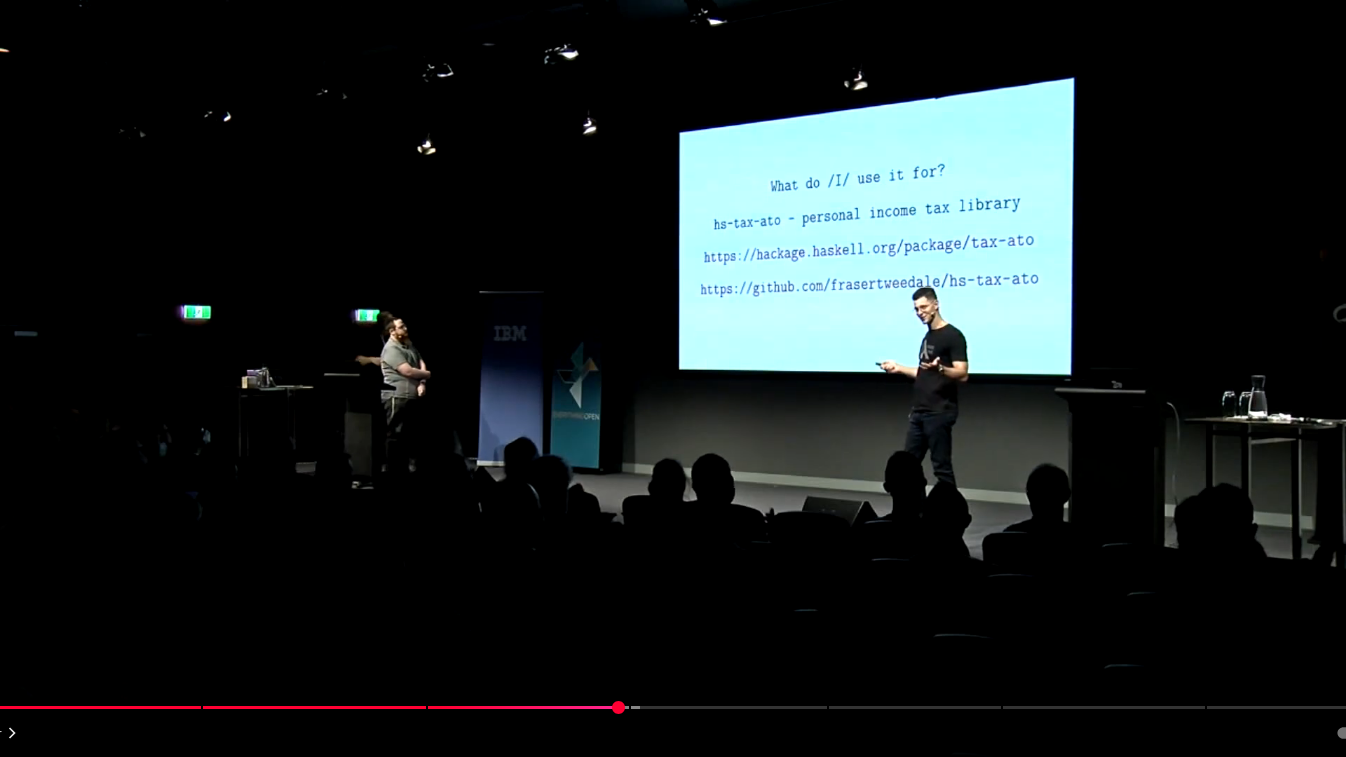
\includegraphics[height=\paperheight,width=\paperwidth]{screenshot.png}
\end{frame}


\begin{frame}[plain]
\Large
\center
\ttfamily
\textbf{ tax-ato - personal income tax library}\\
\bigskip
yes it's Haskell of course, sorry not sorry\\
\bigskip
\url{https://hackage.haskell.org/package/tax-ato}\\
\bigskip
\url{https://github.com/frasertweedale/hs-tax-ato}

\end{frame}

\begin{frame}[plain,fragile]
\tiny
\begin{columns}[t]
  \begin{column}{.5\textwidth}
\begin{verbatim}
import Control.Lens
import Data.Time
import Text.PrettyPrint (render)

import Data.Tax.ATO
import Data.Tax.ATO.CGT
import Data.Tax.ATO.Pretty

import qualified Data.Tax.ATO.FY.FY2024 as FY

main :: IO ()
main = do
  let assessment = assessTax FY.tables taxReturn
  putStrLn . render $ summariseTaxReturnInfo taxReturn
  putStrLn . render $ summariseAssessment assessment

taxReturn :: TaxReturnInfo FY.FY Rational
taxReturn = newTaxReturnInfo
  & set paymentSummaries
      [ PaymentSummary
          "1234567890"      -- ABN
          (Money 180000)    -- Gross payments
          (Money  50000)    -- Tax withheld
          mempty            -- Reportable super contributions
      ]

  & set dividends
      [ dividendFromNetFranked30 -- 30% corporate tax rate
          "IBM"
          (day "2023-09-01")  -- payment date
          (Money 70)          -- net payment
          (proportion 1)      -- franked proportion
      ]
\end{verbatim}
  \end{column}

  \begin{column}{.5\textwidth}
\begin{verbatim}
  & set cgtEvents
      [ CGTEvent
          "NVDA"             -- ticker
          10                 -- units (may be fractional)
          (day "2014-01-01") -- acquisition date
          (Money 30)         -- acquisition price (per unit)
          (Money 20)         -- acquisition cost (brokerage)
          (day "2024-03-01") -- disposal date
          (Money 300)        -- disposal price
          (Money 20)         -- disposal cost
          mempty             -- capital costs
          mempty             -- costs of ownership
      ]

  & set (deductions . workRelatedTravelExpenses) (Money 1000)
  & set (deductions . personalSuperannuationContributions)
      (Money 5000)

  & set helpBalance (Money 10000)

  & set privateHealthInsurancePolicyDetails
      [ PrivateHealthInsurancePolicyDetail
          "NIB"
          "98765432"  -- policy number
          (Money 750) -- premiums eligible for rebate
          (Money 180) -- rebate received
          BenefitCode30
      , PrivateHealthInsurancePolicyDetail
          "NIB" "98765432" (Money 250) (Money  60) BenefitCode31
      ]
\end{verbatim}
  \end{column}

\end{columns}
\end{frame}

\begin{frame}{stuff that was implemented in 2023}
\begin{itemize}
  \item PAYG income, deductions
  \item Medicare levy, Medicare levy surcharge
  \item dividends and franking credits
  \item CGT, foreign income, FITO, ESS
  \item student loan repayments (HECS/HELP/etc)
  \item offsets: LITO, LMITO, spouse super contribution
  \item private health insurance rebate adjustments
  \item rates/rules for previous financial years (back to 2017)
\end{itemize}
\end{frame}

\begin{frame}{stuff that's new since 2023}
\begin{itemize}
  \item PAYG instalments
  \item depreciation schedules
  \item pretty printing
  \item improvements to dividends
  \item vastly expanded documentation and examples
\end{itemize}
\end{frame}

\begin{frame}{stuff that I SHALL implement this year}
\begin{itemize}
  \item personal services income (PSI)
  \item trust distributions
  \item cents-per-kilometer travel expense rates
  \item WFH running costs cents-per-hour rates
\end{itemize}
\end{frame}

\begin{frame}{stuff that's still not implemented}
\begin{itemize}
  \item some adjustments/variations based on family income or dependents
  \item employment termination payments
  \item super income streams and lump payments
  \item rental income and deductions
  \item FHSS releases
  \item some grandfathering rules (e.g. CGT indexation method)
  \item lots of other esoteric (to me) features and quirks
\end{itemize}
\end{frame}

\begin{frame}{want to contribute? (low-hanging fruit)}
\begin{itemize}
  \item rental income and deductions
  \item pre-2017 rates and thresholds
  \item tests
  \item scratch your own itch...
\end{itemize}
\end{frame}


\end{frame}
\begin{frame}[plain]
\centering
\Large
  give it a go, let me know what's missing
\end{frame}


% END MATTER

\begin{frame}[plain]
\begin{columns}

  \begin{column}{.6\textwidth}

    \setlength{\parskip}{.5em}

    { \centering

    \input{cc-by-ARTIFACT.pdf_tex}

    \copyright~2025  Fraser Tweedale

    { \scriptsize
    Except where otherwise noted this work is licensed under
    }
    { \footnotesize
    \textbf{http://creativecommons.org/licenses/by/4.0/}
    }

    }

    \begin{description}
      \item[Code] \url{https://github.com/frasertweedale}
      \item[Blog] \href{https://frasertweedale.github.io/blog-fp/}{frasertweedale.github.io/blog-fp}
      \item[Fediverse] \href{https://functional.cafe/@hackuador}{@hackuador@functional.cafe}
    \end{description}
  \end{column}

\end{columns}
\end{frame}

\end{document}
